\documentclass[aps,prb,amsmath,amssymb,11pt]{revtex4-1}
%\documentclass[journal=ancac3,layout=twocolumn,manuscript=article]{achemso}

\newcommand*{\ACSNANO}{}

\usepackage{chemformula} % Formula subscripts using \ch{}
\usepackage[T1]{fontenc} % Use modern font encodings
\usepackage{graphicx}% Include figure files
\usepackage{dcolumn}% Align table columns on decimal point
\usepackage{bm}% bold math
\usepackage{hyperref}% add hypertext capabilities
% \hypersetup{colorlinks=true,urlcolor={blue},citecolor={blue}, linkcolor={blue}}
\usepackage{amsmath} % or simply amstext
%\newcommand{\angstrom}{\textup{\angstrom}}
\usepackage{siunitx}
\usepackage{color}
\usepackage[normalem]{ulem}
\usepackage{diagbox}
\usepackage{import}
\usepackage{multirow}
\usepackage{xr} % referencing across multiple files
\usepackage{cleveref} % cite figures in SI

\usepackage[normalem]{ulem} %cross out the text, can be deleted later


\newcommand{\comm}{\color{purple}} %comment
%\newcommand{\comm}{\color{green}} %comment

\newcommand{\sinfo}{Supporting Information}
% Use Supp Info labels with SI- prefix
\externaldocument[SI-]{SI}



\ifdefined\INTERNAL

\newcommand{\lock}{\color{red}}
\newcommand{\zhzh}{\color{blue}}

\else

\newcommand{\lock}{\color{black}}
\newcommand{\zhzh}{\color{blue}}




\begin{document}

\title
{Adatoms in the Surface-Confined Ullmann Coupling of Phenyl Groups}

\author{Zhenzhe Zhang}
\author{Dmitrii F. Perepichka}%
\email{dmitrii.perepichka@mcgill.ca}
\author{Rustam Z. Khaliullin}
\email{rustam.khaliullin@mcgill.ca}
\affiliation{%
 Department of Chemistry, McGill University, 801 Sherbrooke St West, Montreal, QC H3A 0B8, Canada
}%

%RZK: Check numbers Au/clean surface - surprisingly similar to Ag.

\begin{abstract}
%\textbf{Abstract.} 
The on-surface Ullmann coupling of aromatic molecules has emerged as the most successful approach to synthesize atomically precise carbon nanostructures with unique electronic properties including molecular wires, graphene nanoribbons and two-dimensional conjugated polymers. Despite substantial progress in determining the mechanism of this reaction, the most fundamental question of whether the coupling is catalyzed directly by surface atoms or adatoms remains unanswered. In this work, the feasibility of the adatom creation and adatom-catalyzed Ullmann coupling of  iodo-, bromo- and chlorobenzene on Cu(111), Ag(111) and Au(111) surfaces is examined using density functional theory modeling. Analysis of competing pathways reveals that two phenyl intermediates extract a silver atom from Ag(111) surface faster (energy barrier 0.43 eV) than they form the carbon-carbon bond (0.62 eV). However, on Cu(111) and Au(111), the extraction process is slower (0.71 eV Cu, 0.36 eV Au) than the C--C formation (0.49 eV Cu, 0.14 eV Au). The adatom creation is greatly facilitated by the strengthening of phenyl-metal bonds upon the extraction. However, if these bonds are too strong they create an insurmountable barrier for the subsequent adatom-catalyzed C--C coupling, as on Cu(111) and Ag(111) (1.78 eV Cu, 1.52 eV Ag). In contrast, Au adatoms that do not bind phenyl groups strongly can catalyze the C--C bond formation almost as efficiently (0.20 eV) as surface atoms (0.14 eV). Our results explain why adatoms are difficult to observe during surface-confined reactions and how their presence can lead to defects in the assembled nanostructures. The revealed trends can facilitate design of efficient on-surface reactions.
%\textbf{Keywords.} Ullmann coupling; surface-confined polymerization; adatom; surface defect; coinage metal; density functional theory.
%\begin{figure}[h!]
%\centering
%\caption{Table of content graphics.} 
%\label{fig:tog}
%\end{figure}

%\vspace{4ex}
\begin{center}
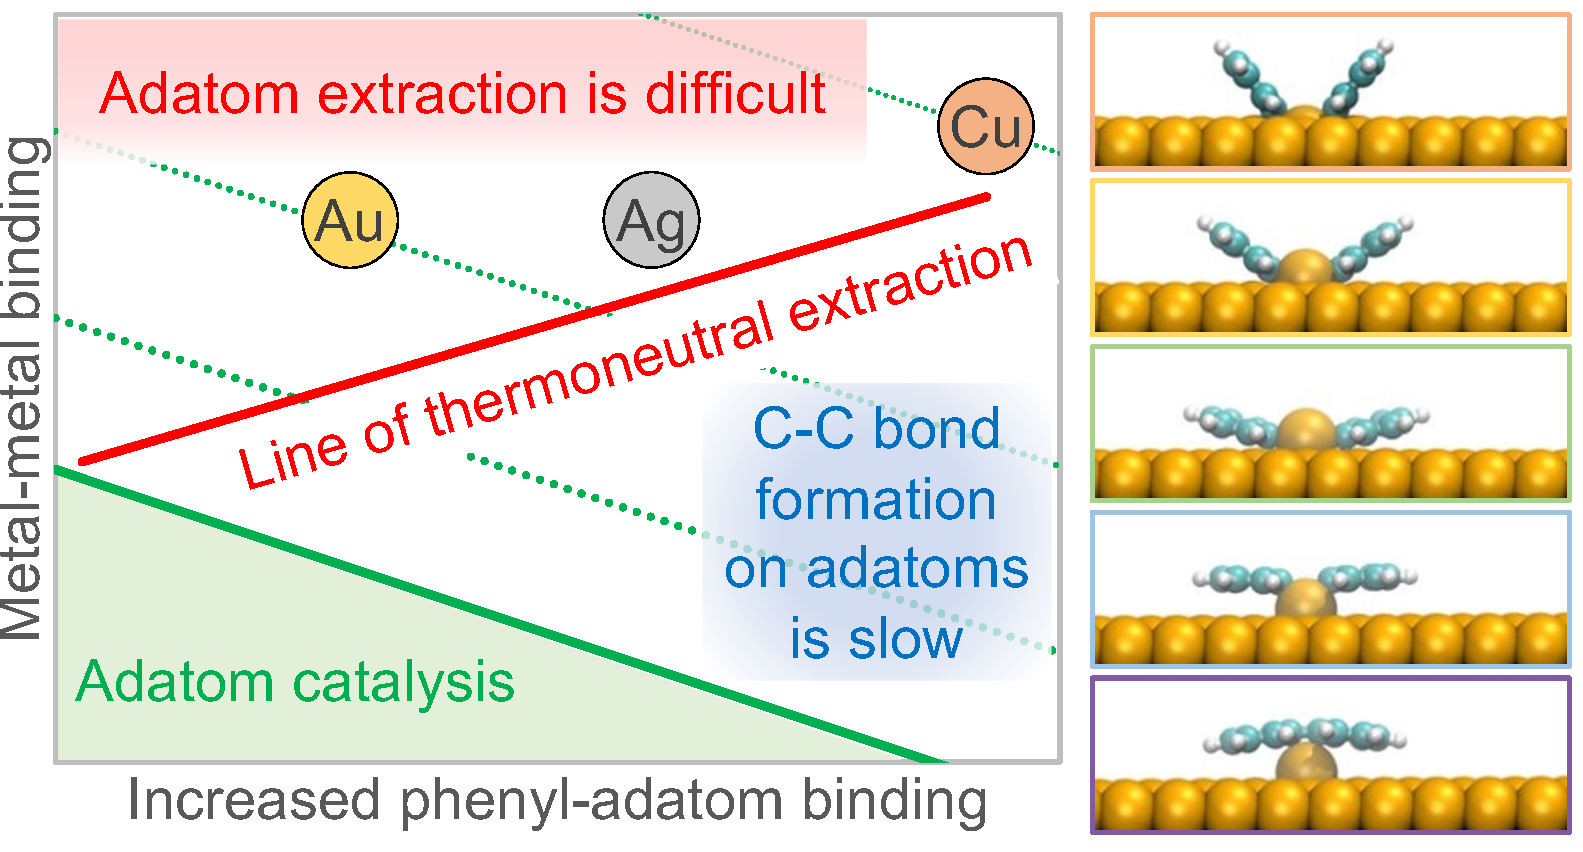
\includegraphics[width=0.50\textwidth]{TOG/TOG-main.pdf}
\end{center}

\end{abstract}


\maketitle

%\section{Introduction}

Unique and tunable properties of $\pi$-conjugated nanomaterials such as graphene nanoribbons~\cite{ullmann_106, ullmann_45, ullmann_107, ullmann_101, Ullmann_153} and two-dimensional conjugated organic polymers~\cite{Ullmann_154, ullmann_148, Ullmann_156, Ullmann_157, Ullmann_158, Ullmann_159, Ullmann_160, Ullmann_161, Ullmann_162, Ullmann_163, Ullmann_164} make them promising candidates for a variety of electronic and optoelectronic devices. Practical applications of these materials in devices requires scalable methods to create extended structures with low defect density.
The Ullmann coupling of aryl halides on metal surfaces -- copper, silver and gold -- is currently the most promising bottom-up strategy to assemble atomically precise $\pi$-conjugated carbon nanostructures with high degree of control over their electronic properties~\cite{ullmann_33, ullmann_42, ullmann_43, ullmann_45, ullmann_46,ullmann_47, ullmann_140, ullmann_148, ullmann_149, ullmann_98, jacs2016, ullmann_152}. 

The mechanism of the surface-confined Ullmann coupling has been studied with a variety of experimental techniques including scanning tunneling microscopy (STM), atomic force microscopy (AFM) and temperature-programmed reaction spectroscopy~\cite{sur_sci01, Ullmann_165, Ullmann_166, Ullmann_167, ullmann_143, ullmann_88,  ullmann_141, ullmann_142, ullmann_87, sur_sci02, ullmann_144}. Experimental investigation is often augmented by computer modeling crucial for interpreting ambiguous experimental data.
It is widely accepted that aryl halide molecules physisorbed on a metal surface dissociate with the formation of surface-bound halogens and aryl groups~\cite{ullmann_145, sur_sci01, ullmann_87, sur_sci03}. The aryl intermediates diffuse on the surface and, once sufficiently close to each other, combine with the formation of an organometallic carbon-metal-carbon bridge structure. This intermediate undergoes reductive elimination to form a covalent carbon-carbon bond between the two aryls. 

Although substantial progress has been made elucidating the mechanism of the Ullmann coupling, our knowledge of several details remains incomplete. Experimental data has been interpreted based almost exclusively on models that describe metal surfaces as ideal, perfectly ordered structures. 
%
Metal surfaces, however, are not free of defects. These defects range from three-dimensional defects such as pores~\cite{ullmann_72} and cracks~\cite{ullmann_73} to planar defects such as twin boundaries~\cite{ullmann_74} and stacking faults~\cite{ullmann_75}, line defects such as dislocations~\cite{Ullmann_76} and to point defects such as adatoms~\cite{Ullmann_77} and vacancies~\cite{ullmann_78}.
%
\sout{It is well known that adatoms are created on clean copper, silver and gold surfaces~\cite{ullmann_79, ullmann_58}, especially near terrace edges and kinks~\cite{ullmann_84, ullmann_85}, in the process of the thermal motion of metal atoms. 
%It has been calculated~\cite{chemeurope2017} that the formation of an adatom on clean Cu(111), Ag(111) and Au(111) surfaces requires substantial energy: \SI{1.71}{\electronvolt}, \SI{1.12}{\electronvolt} and \SI{1.15}{\electronvolt}, respectively. Such high formation energies result in the extremely small equilibrium concentration of adatoms on clean surfaces.  
Although the equilibrium concentration of adatoms on clean surfaces is expected to be extremely small due to the high energy of their formation~\cite{chemeurope2017}, such pre-existing adatoms have been known to participate in metal organic coordination networks~\cite{ullmann_80, ullmann_81, ullmann_82, ullmann_83}.}
{\zhzh Although the equilibrium concentration of adatoms on ideal surfaces is expected to be  small due to the high energy of their formation~\cite{chemeurope2017}, such pre-existing adatoms have been known to form on copper, silver and gold surfaces~\cite{ullmann_79, ullmann_58} near terrace edges and kinks~\cite{ullmann_84, ullmann_85, ullmann_171}. These adatoms have also been found to participate in metal organic coordination networks~\cite{ullmann_80, ullmann_81, ullmann_82, ullmann_83, ullmann_170}.}
There is also a growing body of evidence that adatoms can be created in the process of on-surface reactions~\cite{ullmann_146, ullmann_53, chematerial2019, ullmann_147, chemeurope2017, ullmann_98, ullmann_91}. % indicating that they may also play a role in the surface-confined Ullmann coupling.
%In the process of the Ullmann coupling, reactants, intermediates and final products interact directly with metal atoms on the surface and, therefore, can be affected by surface defects. 
Quantifying the extent to which adatoms and other imperfections of the metal surface influence the thermodynamics and kinetics of the Ullmann coupling can inform new strategies for reaction optimization, leading, in turn, to better defect-free assembly of two-dimensional polymers. 

It has been recently suggested based on results of an STM and density functional theory (DFT) investigation of the on-surface Ullmann coupling reaction that metals atoms bonded to one iodine and one phenyl fragments -- the products of the dehalogenation of a iodobenzene molecule -- can be lifted from their ideal-surface positions and placed onto the surface~\cite{chemeurope2017}. 
The energy required for this extraction has been calculated to be \SI{0.88}{\electronvolt}, \SI{0.53}{\electronvolt} and \SI{0.35}{\electronvolt} for Cu(111), Ag(111) and Au(111) surfaces -- noticeably lower than the \SI{1.71}{\electronvolt}, \SI{1.12}{\electronvolt} and \SI{1.15}{\electronvolt} extraction energies, respectively, on clean surfaces~\cite{chemeurope2017}. %, if the extracted adatom is bonded to iodine and phenyl fragments -- the products of the dehalogenation of a iodobenzene molecule~\cite{chemeurope2017}. 
%
It has also been estimated that the reduced adatom extraction energy can be partially compensated by the release of energy in the preceding dehalogenation step~\cite{chemeurope2017}. %, making the combined dehalogenation and extraction essentially thermoneutral on these surfaces.

The role of adatoms has also been investigated for another step of the Ullmann coupling: the formation of carbon-metal-carbon bridge structures~\cite{acsnano2017, jpcc2018, acsnano2019}. 
%The attention to adatoms in this step stems from the realization that the force exerted upon a metal atom by two aryl radicals is sufficiently strong to lift it high above its ideal-surface position. 
For example, DFT modeling shows that two fluoranthenyl groups lift their shared gold atom \SI{2.2}{\angstrom} above its ideal surface position, which is noticeably higher than the \SI{0.5}{\angstrom} raise produced by a single group~\cite{jpcc2018} and almost equal to the 
%\SI{1.4}{\angstrom} radius of Au atom.
\SI{2.8}{\angstrom} interplanar spacing of Au(111) planes.
The raise of this magnitude suggests that aryl radicals might in principle shift the lifted atom laterally on the surface so it cannot longer recombine with its vacancy. However, such a hypothetical aryl-assisted adatom creation has neither been demonstrated experimentally nor studied computationally.

Pre-existing adatoms have been considered in the case of the formation of the C--M--C bridge from two triphenylene groups on Cu(111) surface. 
The \SI{3.90\pm 0.25}{\angstrom} carbon-carbon distance measured using AFM has been found to agree more closely with the \SI{3.86}{\angstrom} distance calculated for a DFT model with an adatom acting as the bridge rather than with \SI{3.42}{\angstrom} distance calculated for the model with a highly lifted ideal surface atom~\cite{acsnano2017}. 
The close agreement between the measured distance and the former model has been interpreted as evidence of the adatom participation in the Ullmann coupling of bromotriphenylene molecules on Cu(111) surface. 
%
The structural analysis has been supported by the analysis of the energetics of the formation of the C--M--C intermediate from two chemisorbed aromatic groups and an adatom that already exist on the surface. The energy of the formation of the organometallic bridge has been found to be \SI{1.74}{\electronvolt} lower than the energy of the formation of the intermediate on the ideal surface~\cite{acsnano2017}. However, the reported energy difference is not conclusive because the large amount of energy required to create the adatom has not considered.

In another study, a comparison of the twisting angle in experimental and simulated AFM images of the C--M--C intermediates formed by two 4‐bromoterphenyl groups on Cu(111) surface 
has also confirmed that it is an adatom that serves as the metal bridge~\cite{acsnano2019}. Furthermore, an analysis of the temperature-dependent ratio of the two types of C--M--C intermediates that are observed for this precursor has led to a conclusion that the bridge adatoms are extracted during the C--M--C formation step of the surface Ullmann reaction, not simply present on the clean surface before the reaction~\cite{acsnano2019}. 

Unfortunately, the role of adatoms in the formation of the carbon-carbon bond, the final key step of the on-surface Ullmann coupling, has not been investigated. Although the C--C bond formation on a gold atom lifted high above the surface has been studied computationally in the case of bromofluoranthene,
%REVIEW: (Fig.~\ref{fig:high-lift}), 
the investigation focused exclusively on the pathway where the lifted atom returns to its original crystallographic position in the surface~\cite{jpcc2018}. 

Despite the emerging evidence of adatoms being a part of some of the organometallic bridge structures~\cite{acsnano2017, acsnano2019}, it remains unclear whether surface atoms can be extracted by two organic groups. Moreover, it is unknown whether the extracted adatoms can be left behind on the surface, uncoordinated to any groups, after the carbon-carbon bond is formed and, most importantly, whether they can participate in subsequent catalytic coupling cycles.

In order to answer these questions, this work examines, for the first time, the energetics of the adatom creation during the on-surface coupling of two phenyl groups using DFT modeling. 
Furthermore, previously unexplored effects of adatoms, extracted and pre-existing, on the carbon-carbon bond formation between two phenyl groups are investigated in detail. 
The phenyl group, which is produced in the dehalogenation of monosubstituted benzenes, is chosen in this work as the simplest and most studied representative of aromatic building blocks used in on-surface synthesis of carbon nanomaterials. The energetics of all steps of the Ullmann reaction is compared for three different metals (Cu, Ag, Au) and three halogens (Cl, Br, I).

\ifdefined\ACSNANO
\else
\section*{Computational Methods}

The (111) metal surfaces were modeled with slabs containing 192 metal atoms arranged in four 8 $\times$ 6 atomic layers. \SI{10}{\angstrom} of vacuum was added in the direction normal to the surface to ensure weak interaction between periodic images of the slab. The size of the slabs in the lateral directions was $20.55 \times 13.35$~\si{\angstrom} for Cu, $22.84 \times 14.82$~\si{\angstrom} for Ag, and $22.47 \times 14.60$~\si{\angstrom} for Au. It is assumed that the presence of the vacancy does not affect the state energetics drastically and, therefore, the vacancy-containing models are used to model pre-existing adatoms. 

DFT calculations were performed using Vienna \emph{ab initio} simulation package (VASP)~\cite{ullmann_131, ullmann_132, ullmann_133, ullmann_134}. The dispersion-corrected~\cite{ullmann_136, ullmann_137} Perdew-Burke-Ernzerhof (PBE) generalized gradient approximation~\cite{ullmann_139} was used as the exchange-correlation functional. 
Spin-polarized electronic states were modeled using a plane wave basis set with the energy cut-off set at \SI{800}{\electronvolt}.
The projector augmented wave formalism was used to describe interactions of atomic cores with valence electrons. The integration over the Brillouin zone was performed using the $3\times 3 \times1$ Monkhorst-Pack $k$-point mesh. 

Atomic positions were optimized until the maximum force on atoms decreased below \SI{0.02}{\electronvolt\per\angstrom}. 
Transition state structures were located using the climbing-image nudged elastic band (NEB) with the VTST code~\cite{ullmann_59}. 
In NEB calculations, an improved initial guess~\cite{ullmann_60, ullmann_99} for the minimum energy path was used and the positions of atoms were relaxed until the maximum force dropped below \SI{0.1}{\electronvolt\per\angstrom}.

%{\comm RZK0804: Energy vs enthalpy.}

\fi


%\section*{Results and Discussion}

\ifdefined\ACSNANO

Slab models were employed to represent metal surfaces. DFT calculations were performed using the dispersion-corrected~\cite{ullmann_136, ullmann_137} Perdew-Burke-Ernzerhof~\cite{ullmann_139} functional (see Computational Methods for details).
%
\fi
%
The coupling reaction on the Cu(111) surface is discussed in detail first. The coupling on the Ag(111) and Au(111) surfaces are considered in comparison with the Cu(111) surface next.

\begin{figure*}[bt]
\centering
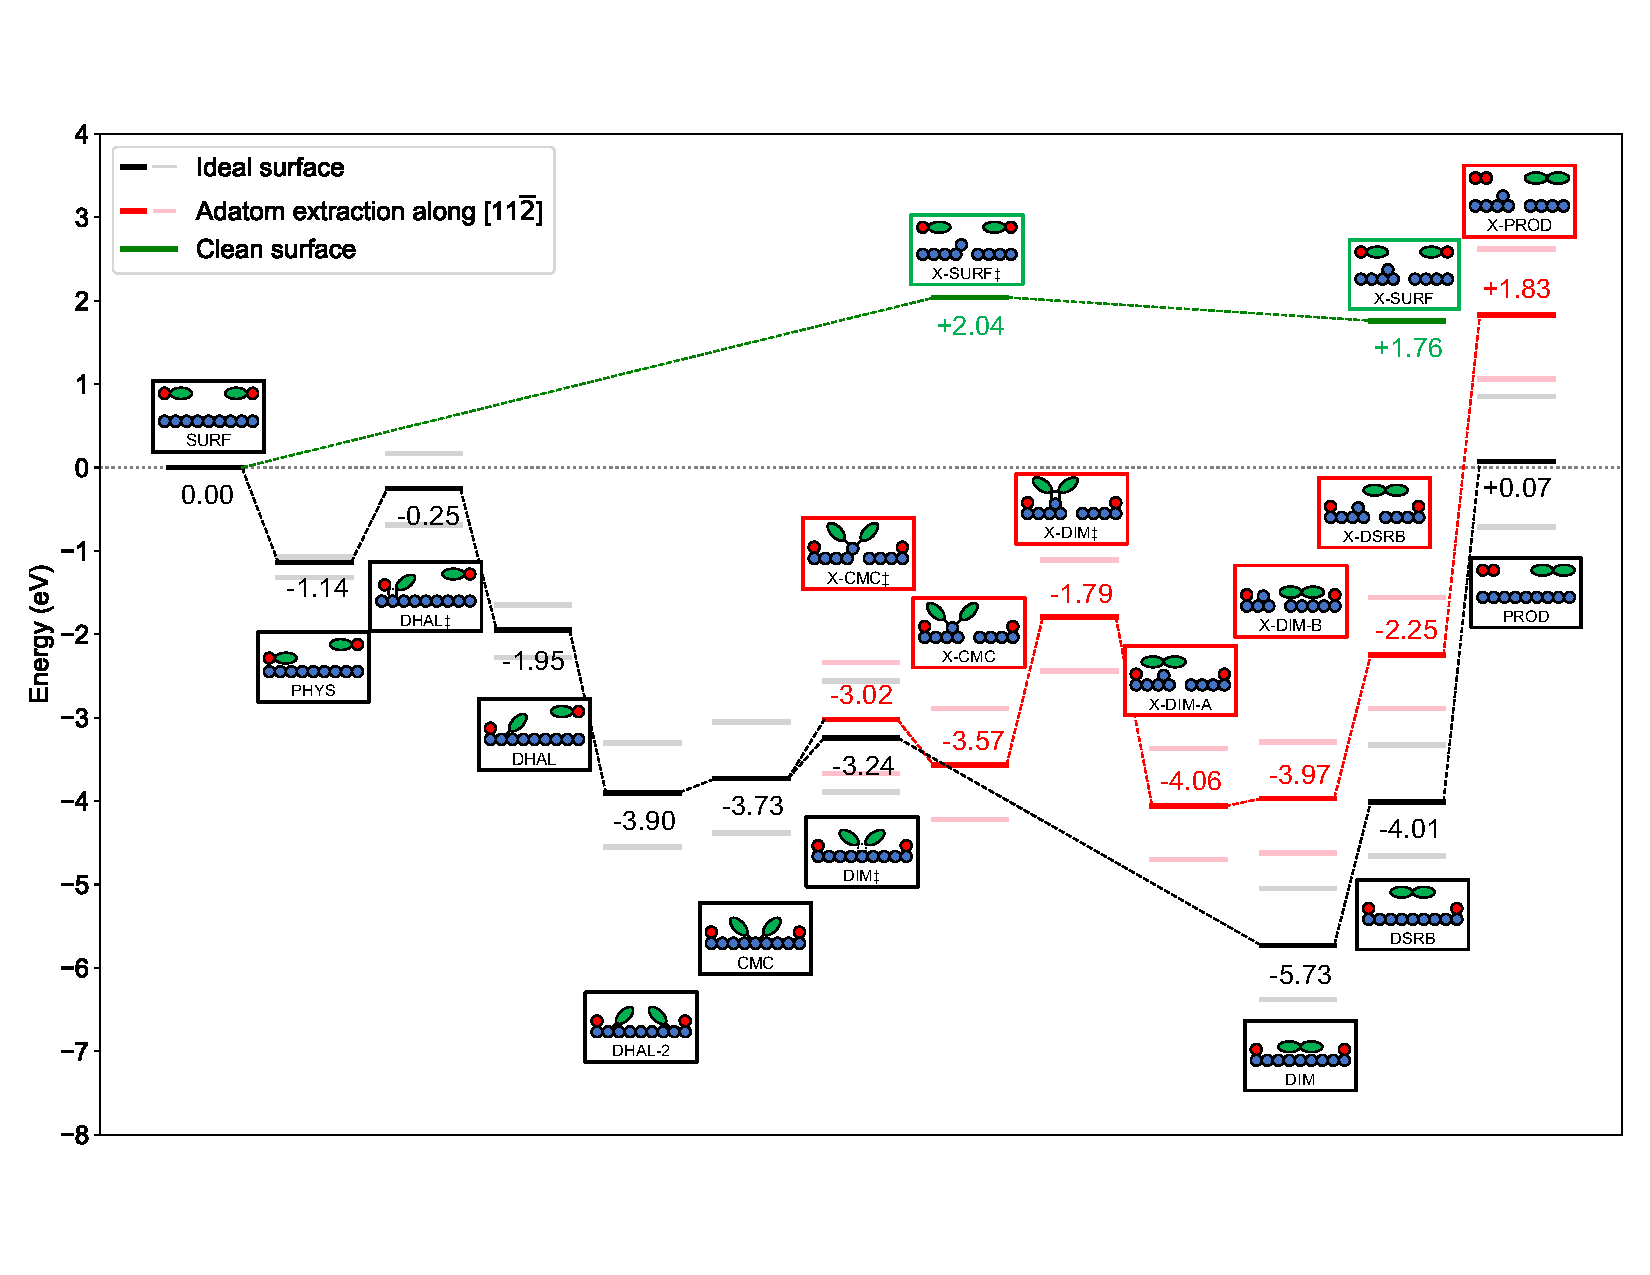
\includegraphics[width=1.\textwidth]{Fig/main-profile.pdf}
\caption{
Energy profile of the Ullmann reaction of monohalogentated benzenes on Cu(111). In the pictograms, blue, red, and e shapes denote copper atoms, halogen atoms, and phenyl groups, respectively. %The energy of the ideal metal surface and two gas-phase monohalogenated benzene molecules, denoted here as \textbf{SURF}, was used as the zero-energy reference. 
Levels shown with bright colors are states with bromine as the halogen, whereas the faint upper and lower levels denote states with chlorine and iodine as the halogen, respectively. It is assumed that halogen atoms do not influence the reaction after the dehalogenation step (but see Refs.~\onlinecite{ullmann_52, Ullmann_168, Ullmann_169}) and, therefore, only the energy levels for bromine containing species are shown. The numerical values of all species are collected in Tables~\ref{SI-table:bondlength}, \ref{SI-table:idealsurface} and~\ref{SI-table:adatom-longitude}. {\zhzh Abbreviation of states: SURF: surface with unadsorbed molecules; PHYS: one physisorbed molecule; DHAL: one dehalogenated molecule; DHAL-2: two dehalogenated molecules; (X-)CMC: (extracted adatom) Carbon-Metal-Carbon bridge intermediate; (X-)DIM: (extracted adatom) dimerized coupling product; X-DIM-A: dimer on adatom; X-DIM-B: dimer product detach; (X-)DSRB: (extracted adatom) only dimer desorbed; (X-)PROD: (extracted adatom) halogens and dimer desorbed}}
\label{fig:completeenergy}
\end{figure*}

\textbf{Ullmann coupling on Cu(111).}
%
%RZZK0816 - modify the last sentence of the intro to remove different halogens? 
%RZZK - reconsider names of subsections.
In the initial steps of the Ullmann reaction (Fig.~\ref{fig:completeenergy}) the halogenated benzene molecules, physisorbed on the metal surface (\textbf{PHYS}), dissociate \sout{with the formation of} {\zhzh forming} the surface-bound phenyl groups (\textbf{DHAL}), which then combine forming organometallic bridge structures (\textbf{CMC}).
The calculated energy profiles of these steps for three halogens (Figs.~\ref{fig:completeenergy}, \ref{SI-fig:dissociation_Br}--\ref{SI-fig:dissociation_I} and Table~\ref{SI-table:bondlength}) are in qualitative agreement with the trends in the experimentally measured onset temperatures of dehalogenation (Table~\ref{SI-table:experimental-temperatures})~\cite{ullmann_52,ullmann_87,ullmann_67} and with the previous calculations on this~\cite{jacs2013,ullmann_88} and similar systems. 

{\zhzh Dima suggests to move to abstract or intro} \sout{The main focus of this work is on the formation of a C--C bond -- the final step of the Ullmann coupling.} 
Two pathways to create the C--C bond are considered here. 
In the first pathway, the bridge Cu atom {\zhzh from \textbf{CMC}} returns to its original position \sout{in the first metal layer} after the C--C bond is formed. This pathway is referred to as the ideal-surface pathway.
In the second pathway, the Cu atom is pulled out \sout{from the topmost metal layer} to become an adatom, leaving a vacancy in its original position. This pathway is called the adatom pathway.

The C--C bond formation along the ideal-surface path is so exothermic (\SI{-2.00}{\electronvolt}) that it can be considered irreversible at the typical temperatures of the Ullmann coupling of phenyl groups on copper (\SI{350}{\kelvin})~\cite{ullmann_67, sur_sci01}. The energies of the initial (\textbf{CMC}), transition (\textbf{DIM$\ddagger$}) and final states (\textbf{DIM}, for biphenyl) along the ideal-surface pathway are shown in Fig.~\ref{fig:completeenergy} whereas their structures and the nudged elastic band (NEB) energy profile are presented in Fig.~\ref{fig:distance-energy}. 
The ideal-surface path has a relatively small \SI{0.49}{\electronvolt} energy barrier, in agreement with previous calculations (Table~\ref{SI-table:idealsurface})~\cite{pccp2010, jacs2013}. %, which in line with the onset temperature for the C--C bond formation from two phenyl radicals on Cu(111) is \SI{300}{\kelvin} in experiment~\cite{sur_sci01}.
Fig.~\ref{fig:distance-energy} and Table~\ref{SI-table:idealsurface} show that, in this pathway, the bridge cooper atom returns back to its position isochronously with the C--C bond formation. 

\begin{figure*}[bt]
\centering
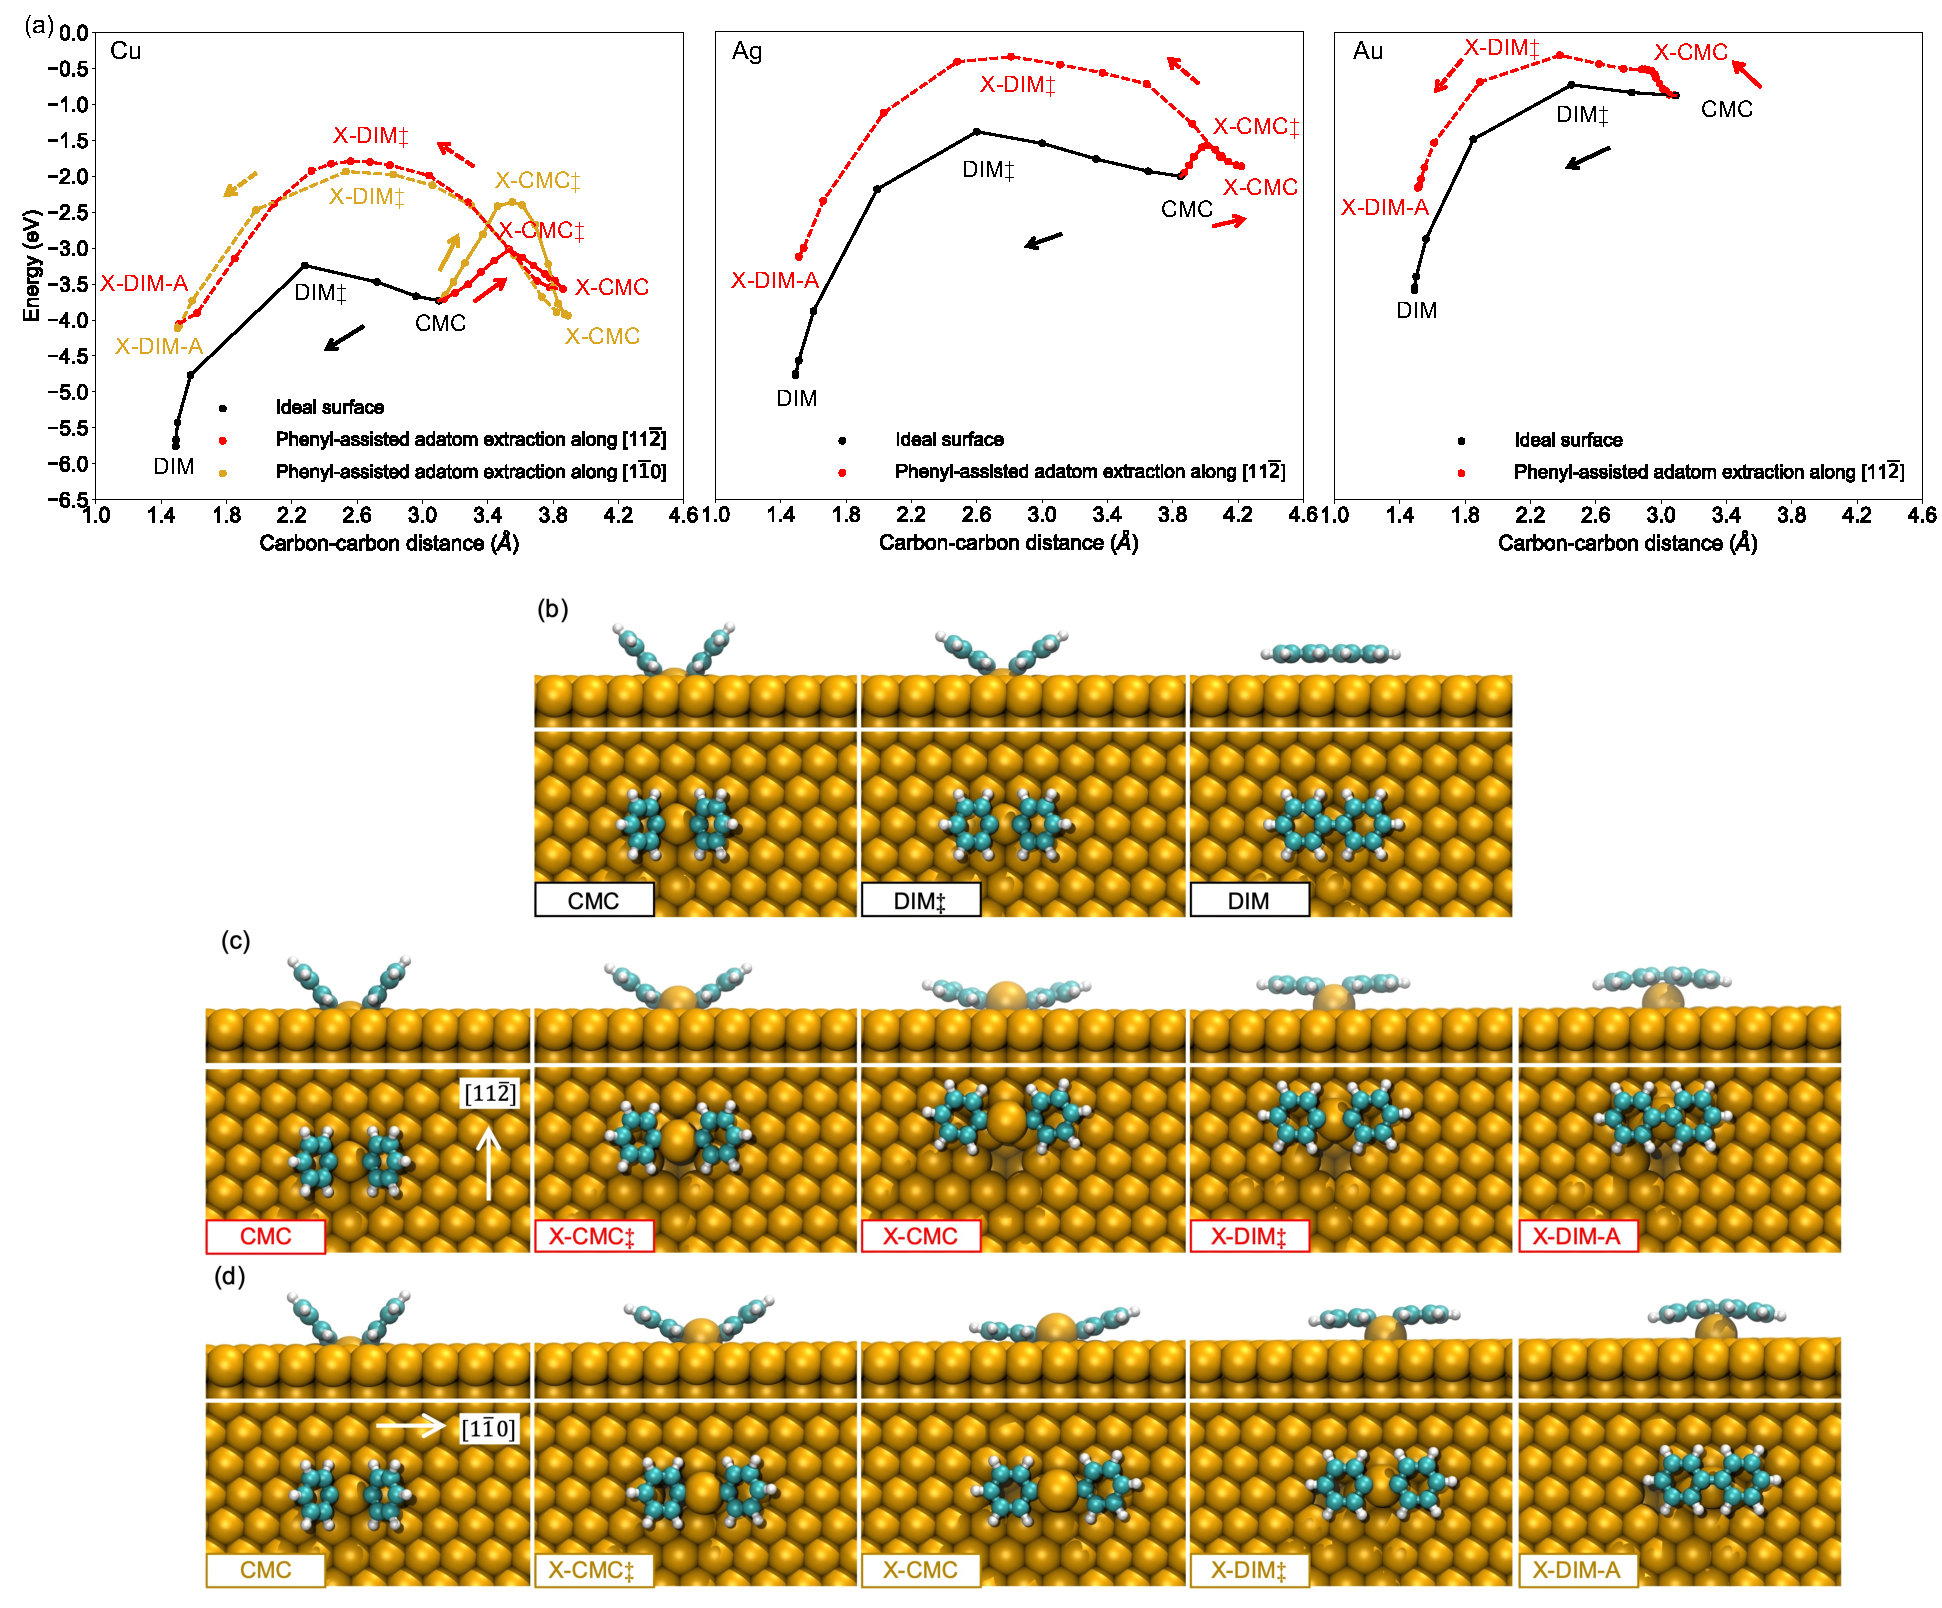
\includegraphics[width=1.0\textwidth]{Fig/distance-energy.pdf}
\caption{Coupling of the phenyl groups along the ideal-surface (black),  [11$\overline{2}$] adatom (red), and  [1$\overline{1}$0] adatom (yellow) pathways. (a) NEB energy profiles along the reaction coordinate represented by the distance between the two carbon atoms. For the Cu(111) surface, the geometry of key intermediates is shown along the (b) ideal-surface, (c) [11$\overline{2}$] adatom, and (d) [1$\overline{1}$0] adatom pathways.}
\label{fig:distance-energy}
\end{figure*}

The adatom pathway consists of three elementary steps: the adatom extraction, the C--C bond formation on the adatom, and the diffusion of biphenyl away from the adatom. 
The adatom extraction was considered along the two high-symmetry surface directions $[1\bar{1}0]$ and $[11\bar{2}]$ (Fig. \ref{fig:distance-energy}) and the product of the extraction -- an adatom bonded to two phenyl radicals -- is denoted \textbf{X-CMC}, where \textbf{X} refers to the presence of eXtracted adatom in this and other state labels. 
The higher stability of the $[1\bar{1}0]$ \textbf{X-CMC} state is most likely due to the stronger interaction between the undercoordinated metal atoms at the vacancy edges and the nearby phenyl ring (Figure~\ref{fig:distance-energy}).
However, the extraction along the $[11\bar{2}]$ direction has lower barrier than that along the $[1\bar{1}0]$ direction (\SI{0.71}{\electronvolt} \emph{vs} \SI{1.38}{\electronvolt}) because the adatom does not have to be lifted as high in the \textbf{X-CMC$\ddagger$} transition state in the former case (\SI{1.58}{\angstrom} \emph{vs} \SI{1.68}{\angstrom}, Table~\ref{SI-table:adatom-longitude}). This difference in the barrier height is significant enough to consider only the $[11\bar{2}]$ extraction further.
{\zhzh Two possibilities of adatom catalyzed C--C formation were also explored: successive or simultaneous occurrence of C--C formation and adatom diffusion. The energy barrier of the latter is so high (\SI{3.04}{\electronvolt}) that the path adatom diffusion after C--C formation is taken in count further (Fig. ~\ref{fig:AlterPath})}.

\begin{figure*}[bt]
\centering
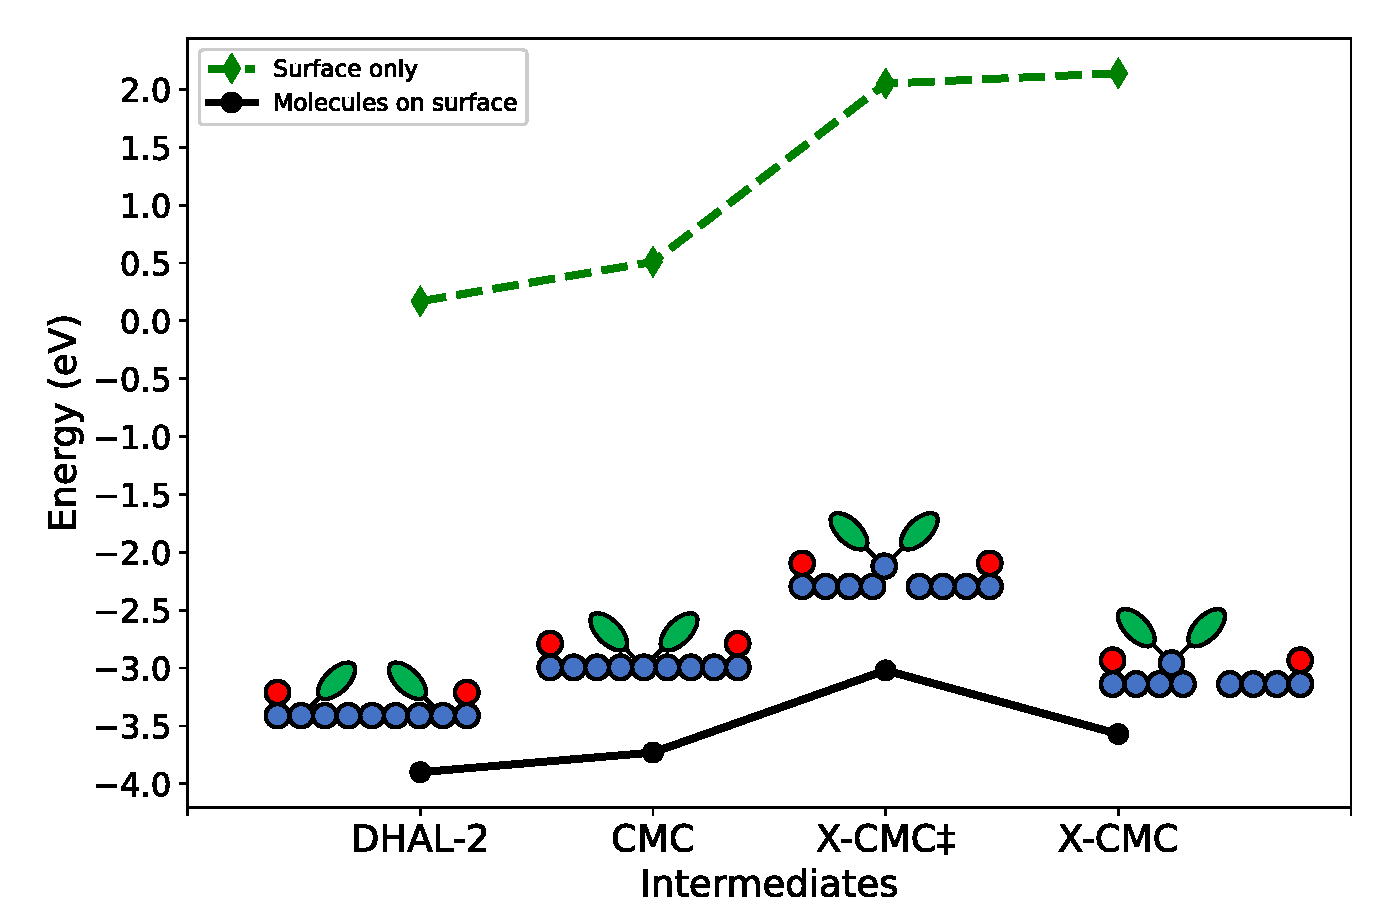
\includegraphics[width=0.95\textwidth]{Fig/onlysurface.pdf}
\caption{
(a) The strength of the interaction energy between the two phenyl groups and copper {\zhzh, silver and gold} surface, measured as the change from the \textbf{CMC} state. (b) Dependence between the decreased catalytic activity of adatoms and strengthening of the phenyl-adatom binding. In both axis labels, $\Delta$ refers to the change from the ideal suface to adatom. The linear trendline enforced to go through the origin is $y=0.898 x$ ($R^2 = 0.950$).}
\label{fig:onlysurface}
\end{figure*}

It is remarkable that the energy of the extraction of a copper atom bonded to two phenyl groups is only \SI{0.16}{\electronvolt} -- dramatically lower than the \SI{1.76}{\electronvolt} energy required to extract an adatom \sout{from the ideal clean surface} {\zhzh in an unassisted extraction fashion} (green pathway in Fig.~\ref{fig:completeenergy}). The \SI{0.71}{\electronvolt} barrier height for the phenyl-assisted extraction is also substantially lower than the \SI{2.04}{\electronvolt} barrier of unassisted extraction, due to the increased binding of the phenyl groups to the Cu adatom (Fig.~\ref{fig:onlysurface}a). This strengthening is also manifest in the \SI{0.12}{\angstrom} decrease in the carbon-metal bond length during the \textbf{CMC} to \textbf{X-CMC} transformation (Table~\ref{SI-table:adatom-longitude}).

It is also worth noting that the adatom extraction assisted by two phenyl groups requires less energy {zhzh (\SI{0.16}{\electronvolt})} than the previously described extraction assisted by a single phenyl group and a halogen atom {\zhzh \SI{0.88}{\electronvolt}~\cite{chemeurope2017}.} \sout{, which can happen immediately after the dehalogenation step~\cite{chemeurope2017}.} \sout{In the previous study~\cite{chemeurope2017}, which used different slab models and different density functional, the energy of the extraction of a copper atom assisted by phenyl and iodine was calculated to be }\SI{0.88}{\electronvolt} (cf. \SI{0.16}{\electronvolt} \sout{phenyl-assisted extraction here).}

With the permissive energetics of adatom extraction, it is important to look closely into the formation of the C--C bond catalyzed by the adatom (\textbf{X-CMC}, \textbf{X-DIM$\ddagger$}, \textbf{X-DIM-A}).
In contrast to the C--C bond formation on the ideal surface, the energy release along this step of the adatom pathway is moderate \SI{-0.48}{\electronvolt} (\textit{cf.} \SI{-2.00}{\electronvolt} on the ideal surface) while the barrier height is the prohibitive \SI{1.78}{\electronvolt} (\textit{cf.} \SI{0.49}{\electronvolt}). 
This difference between the ideal-surface and adatom pathways can be attributed to the strong bonds between the phenyl groups and adatom.
Their cleavage  hinders the C--C bond formation as much as their formation facilitates the extraction step.

It is worth noting that the adatom pathway can also be viewed as a sum of two different steps: the exothermic ideal-surface C--C bond formation (\SI{-2.00}{\electronvolt}) and the energy demanding adatom extraction \sout{on clean surface} unassisted (\SI{1.76}{\electronvolt}). 
The entire pathway is, therefore, nearly thermoneutral (\SI{-0.24}{\electronvolt}). 
\sout{Interestingly, however} {\zhzh In fact}, all three steps along the adatom pathway -- extraction, C--C bond
formation, and the biphenyl diffusion -- are also almost thermoneutral, with their own energy balancing mechanisms (Fig.~\ref{fig:completeenergy}). 
In the first step, the adatom escapes the pull of its metal neighbors with the compensating strengthening of the two phenyl-adatom bonds. In the second step, the strong carbon-adatom bonds are converted into the equally strong C--C bonds without a significant release of energy. Finally, the biphenyl drifts away from the adatom without experiencing a strong resisting force. Despite the permissive thermodynamics, however, the high energy of the transition state in the C--C bond formation step (\textbf{X-DIM$\ddagger$}) renders the biphenyl formation through the \sout{extracted} adatom pathway unlikely.
Moreover, even with the surprising ease of the phenyl-assisted adatom extraction, the organometallic bridges containing extracted adatoms (\textbf{X-CMC}) are unlikely to be observed in STM or AFM experiments. This is because the small fraction of the \textbf{CMC} organometallic bridges that get converted to \textbf{X-CMC} are unable to catalyze the further C--C bond formation and predestined to recombine with the vacancy. In contrast, the competing C--C bond formation on the ideal surface is essentially irreversible, producing the equilibrium mixture heavily dominated by ideal-surface biphenyl molecules.

\textbf{Coupling on pre-existing Cu adatoms.} We also examined the Ullmann coupling catalyzed by the adatoms that are not extracted during the reaction but already exist on the Cu(111) surface. Such pre-existing adatoms are known to form on Cu surfaces due to thermal fluctuations around various defects such as terrace edges and kinks. 
Fig.~\ref{fig:adatomullmann} shows that the Ullmann coupling of surface-bound phenyl groups on a pre-exisitng adatom is a highly exothermic process. Once the carbon-halogen bond is broken (e.g. on the ideal surface) the phenyl groups need to overcome only a minor diffusion barrier~\cite{pccp2010} to move closer to the existing adatom and to form bonds with them. 
Fig.~\ref{fig:adatomullmann} shows the synergistic binding of two phenyl groups to an adatom. While the first phenyl is coordinated to the adatom with the energy release of \SI{0.49}{\electronvolt} {\zhzh (\textbf{X-SING})}, binding of the second phenyl is accompanied by the the release of additional \SI{0.95}{\electronvolt} and the system system becomes trapped in the \textbf{X-CMC} state. On one hand, the C--C bond formation cannot proceed because of the height of the \textbf{X-DIM$\ddagger$} barrier {\zhzh (\SI{1.78}{\electronvolt})}. On the other hand, the reverse dissociation of the strong adatom-phenyl bond also requires at least \SI{0.95}{\electronvolt} of energy. 
Because of such \textbf{X-CMC} traps, the presence of adatoms during the Ullmann-based polymerization on the Cu(111) surface can lead to defects in the assembled nanostructures.

\begin{figure}[bt]
\centering
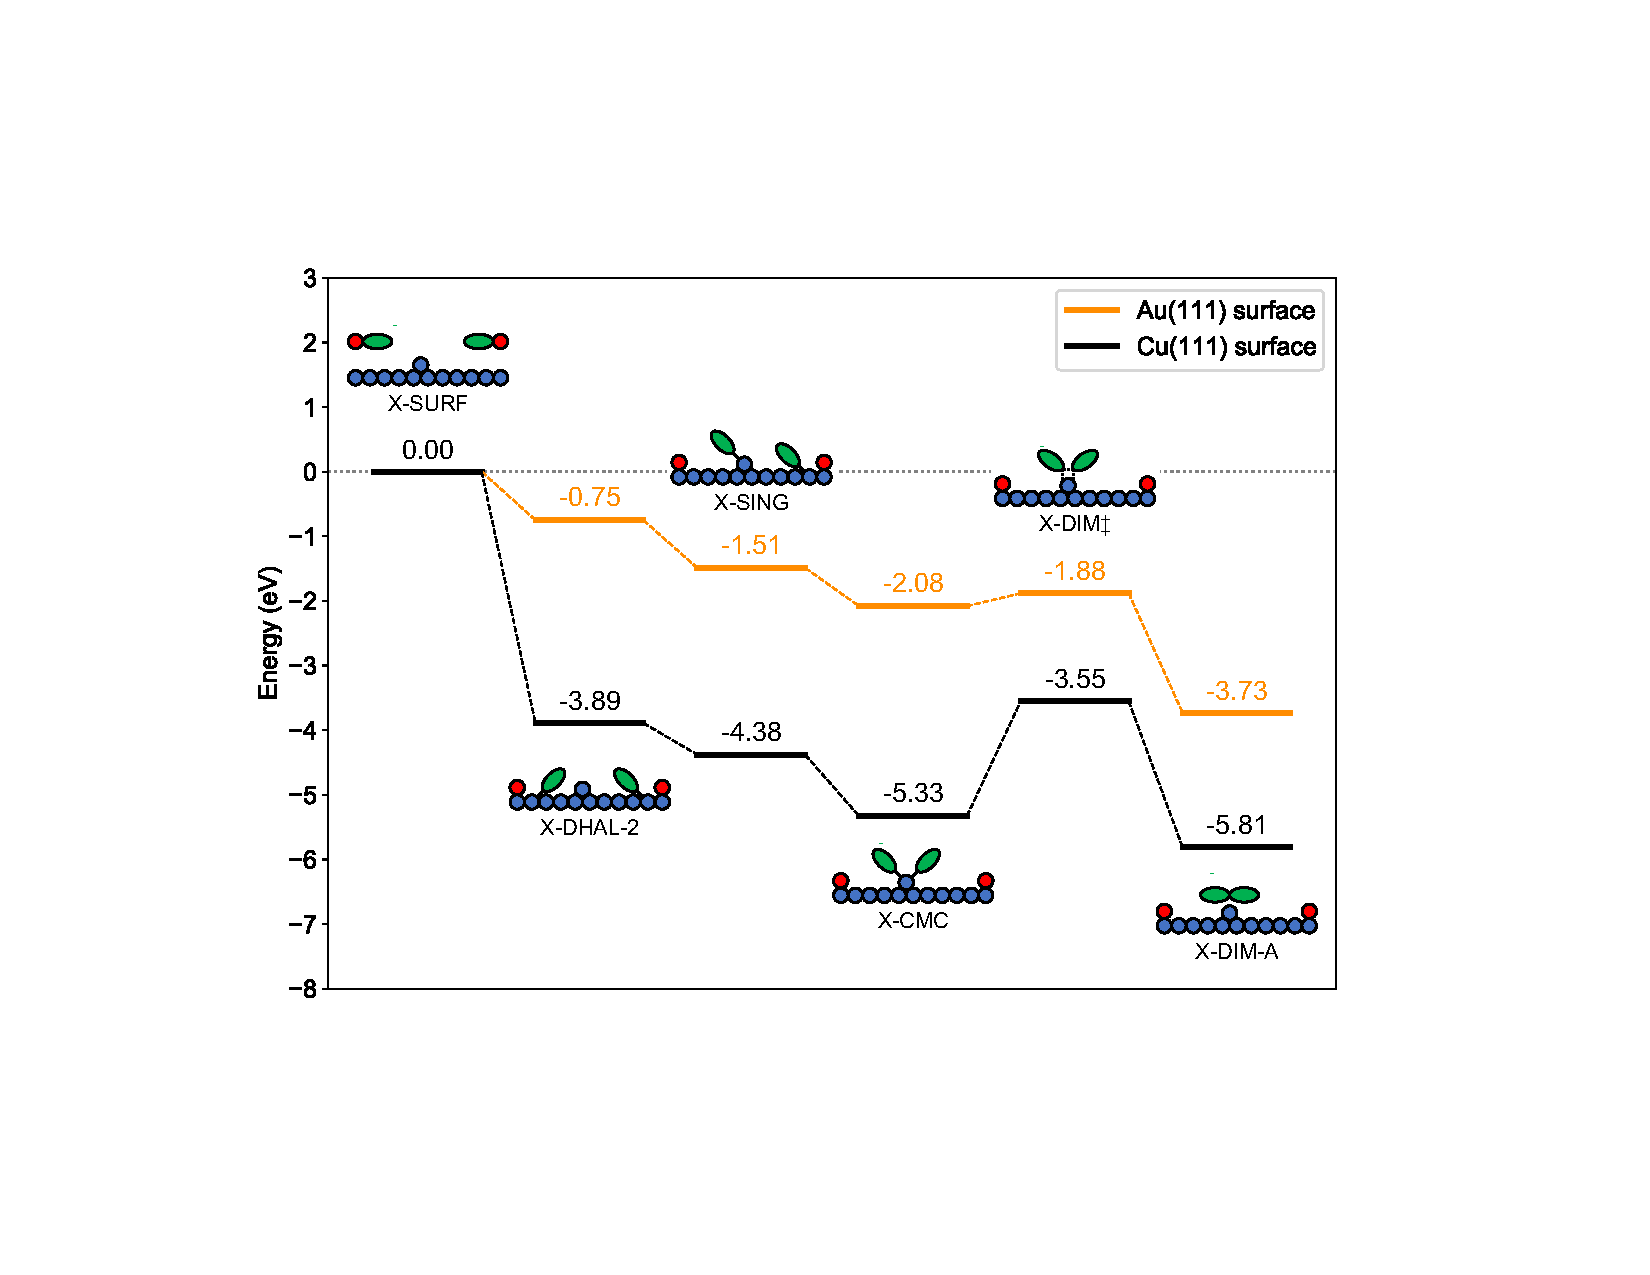
\includegraphics[width=0.48\textwidth]{Fig/ullmann_adatom.pdf}
\caption{Energy profiles of the Ullmann reaction of bromobenzene on pre-existing adatoms on Cu(111) and Au(111) surfaces.}
\label{fig:adatomullmann}
\end{figure}

\begin{figure*}[bt]
\centering
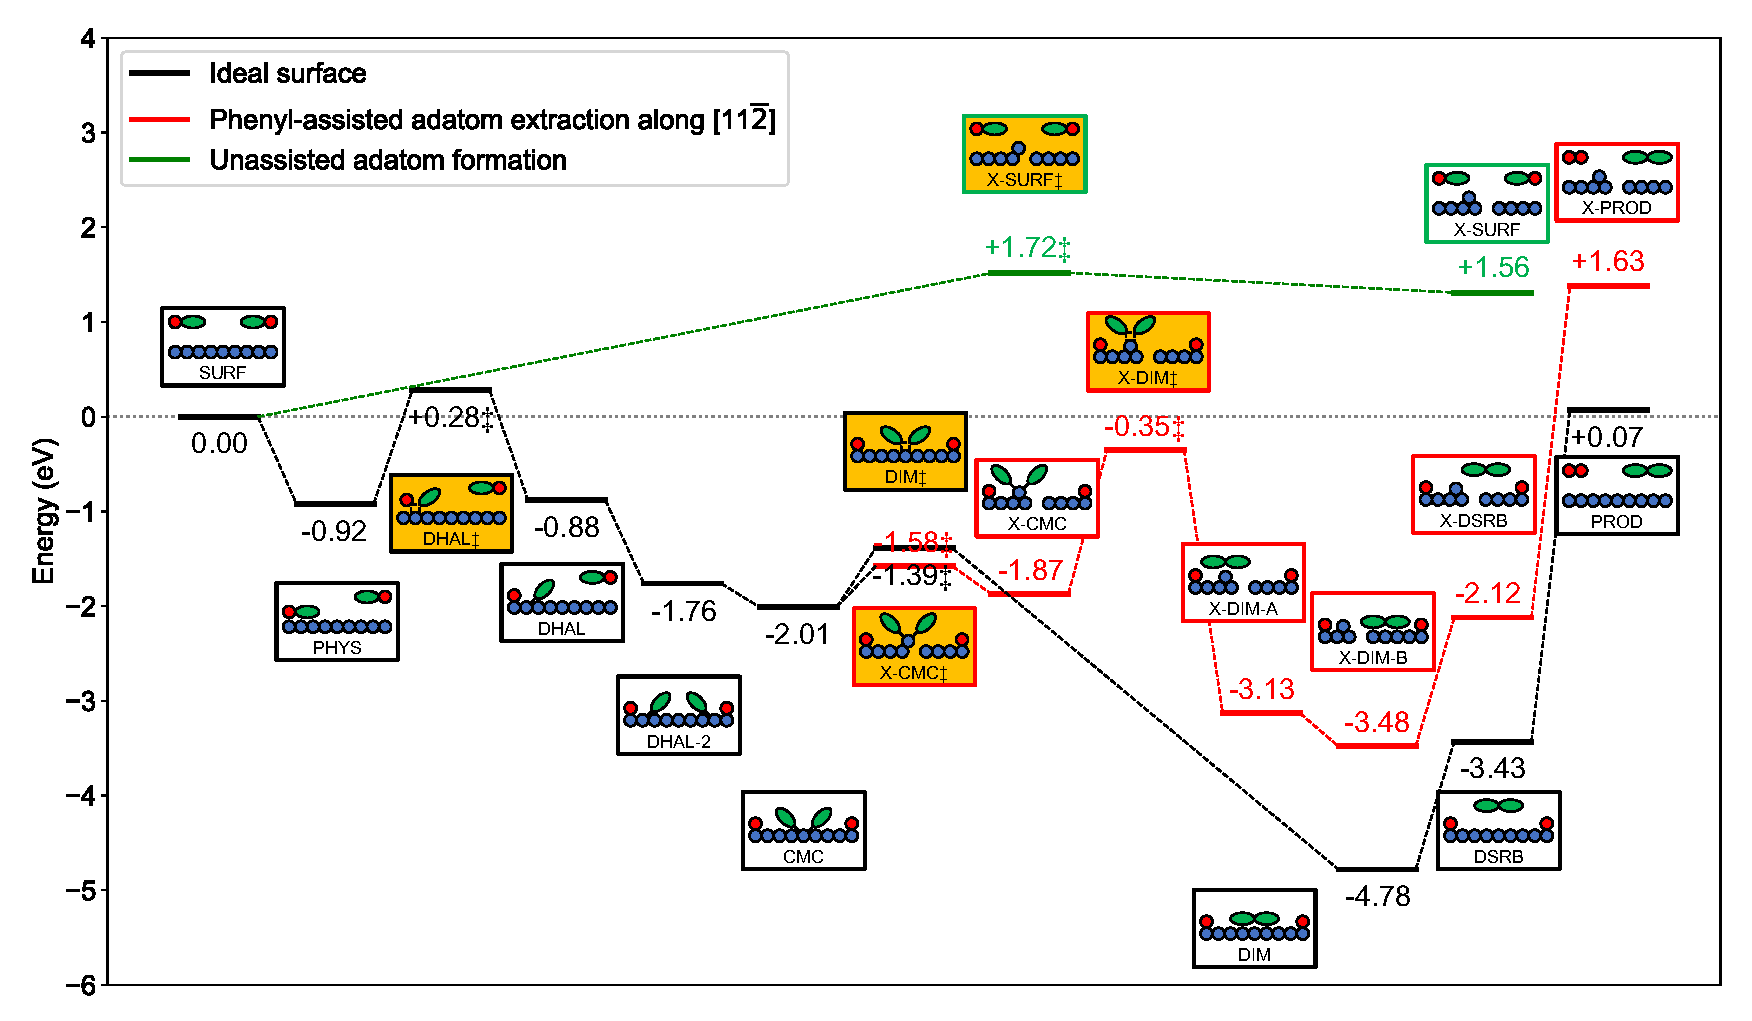
\includegraphics[width=1.\textwidth]{Fig/Ag_mainfile.pdf}
\caption{Energy profile of the Ullmann reaction of bromobenzene on Ag(111).}
\label{fig:Ag_all}
\end{figure*}

\begin{figure*}[bt]
\centering
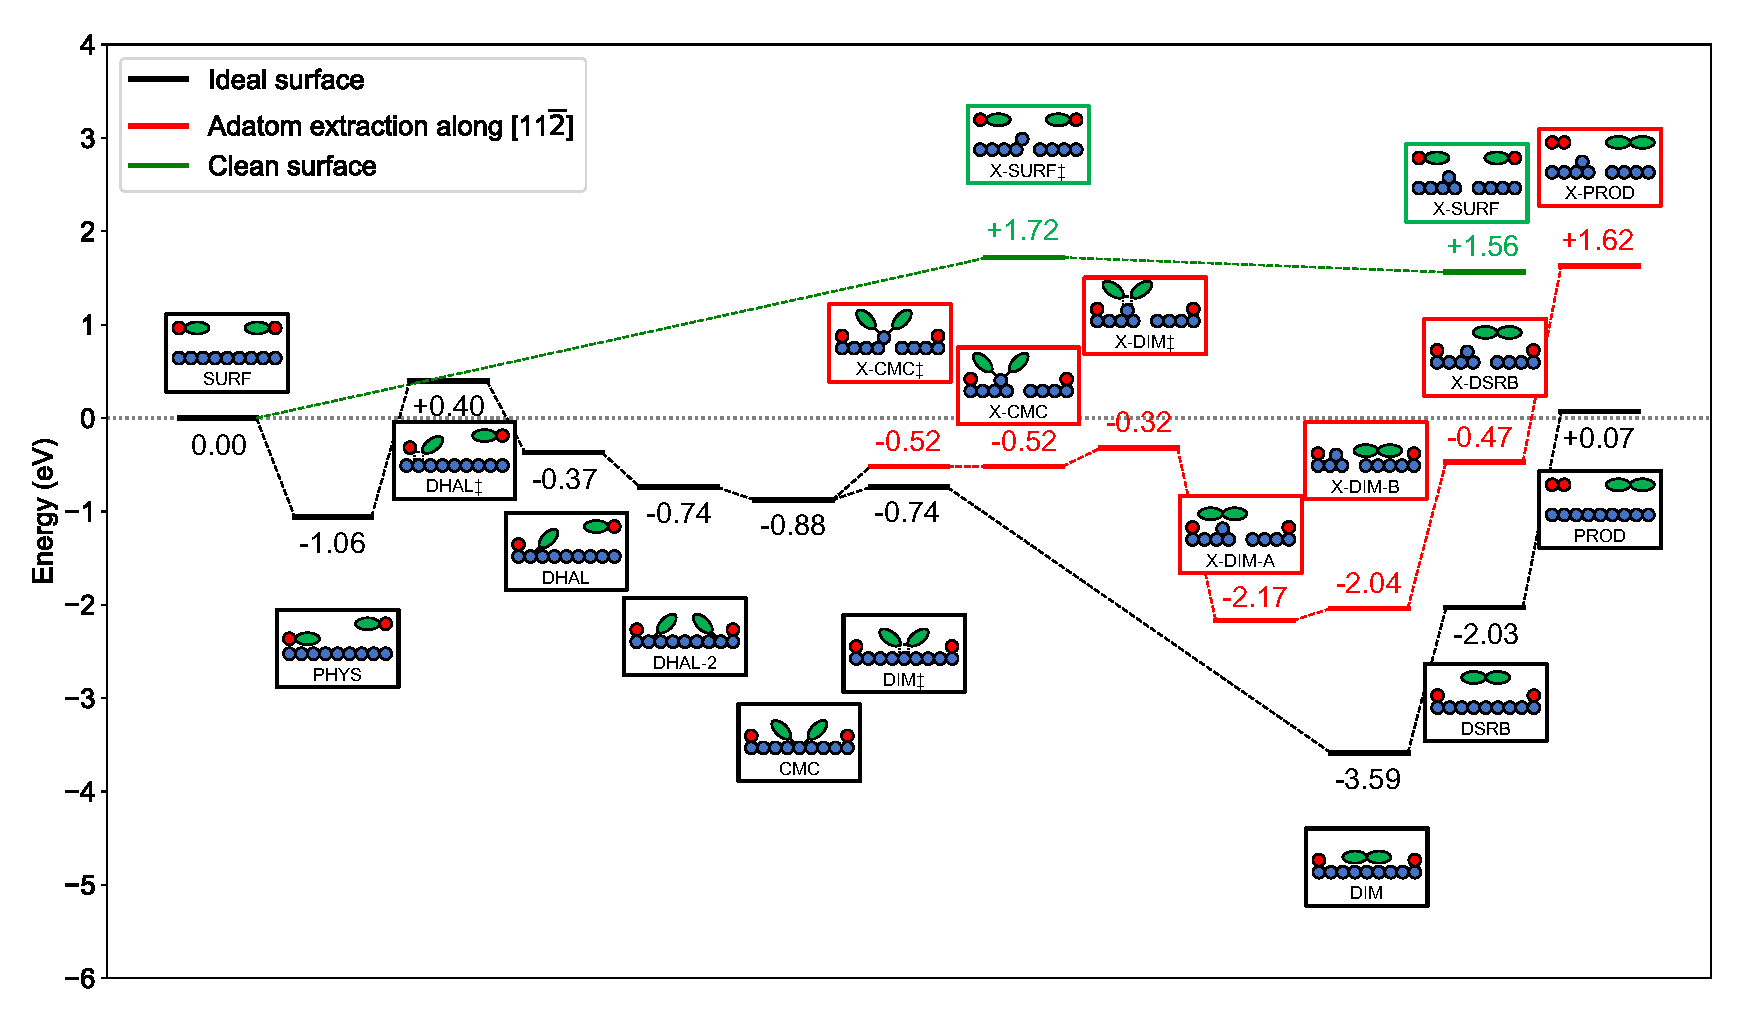
\includegraphics[width=1.\textwidth]{Fig/Au_mainfile.pdf}
\caption{Energy profile of the Ullmann reaction of bromobenzene on Au(111).}
\label{fig:Au_all}
\end{figure*}


\textbf{Ullmann reaction on Ag(111) and Au(111).}
%
Energy profiles of the Ullmann reaction on the ideal Ag(111) and Au(111) surfaces were calculated for bromobenzene (Figs.~\ref{fig:Ag_all} and~\ref{fig:Au_all}). 
The energy barriers of the \sout{debromination step} {\zhzh formation of \textbf{DHAL}} increase from Cu (\SI{0.89}{\electronvolt}) to Ag (\SI{1.20}{\electronvolt}) and to Au (\SI{1.46}{\electronvolt}) in agreement with the trend in the experimentally measured dehalogenation temperatures~\cite{ullmann_52,ullmann_87,ullmann_67} (Table~\ref{SI-table:experimental-temperatures}) and with previous calculations~\cite{jacs2013}.
At the same time, the energy barriers of the C--C formation step (Fig.~\ref{fig:distance-energy}a, Table~\ref{SI-table:idealsurface}) follow a different trend decreasing from Ag (\SI{0.62}{\electronvolt}) to Cu (\SI{0.49}{\electronvolt}) and to Au (\SI{0.14}{\electronvolt}), again in agreement with experimental (Table~\ref{SI-table:experimental-temperatures}) and previously reported DFT~\cite{jacs2013} trends. The adatom pathways on Ag(111) and Au(111) exhibit several interesting features not seen for Cu(111).

First, the phenyl-assisted adatom extraction on Ag(111) surface has a lower activation energy (\SI{0.43}{\electronvolt}) along the $[11\bar{2}]$ pathway and thus proceeds faster than the conventional ideal-surface C--C bond formation (\SI{0.62}{\electronvolt}), in contrast to the Cu-mediated processes (Fig.~\ref{fig:distance-energy}a). However, despite the fast formation of the phenyl-bonded adatoms on Ag(111), the fate of these species is the same as those on Cu(111): silver adatoms quickly recombine with their vacancies and the biphenyl formation occurs along the conventional ideal-surface pathway, which has a lower activation barrier (\SI{0.62}{\electronvolt}) than that of adatom-catalyzed coupling (\SI{1.52}{\electronvolt}).

Second, the barrier of the adatom-catalyzed C--C formation on Au (\SI{0.20}{\electronvolt}) is dramatically lower than those for Ag (\SI{1.52}{\electronvolt}) and Cu (\SI{1.78}{\electronvolt})  (Fig.~\ref{fig:distance-energy}a). 
However, when the additional \SI{0.36}{\electronvolt} barrier of the Au atom extraction is taken into account, it is clear that
the transformation along the adatom pathway is significantly slower at the typical temperatures of the Ullmann reaction on Au (Table~\ref{SI-table:experimental-temperatures}) than the rapid C--C bond formation on the ideal surface with its \SI{0.14}{\electronvolt} activation energy. 
Since the extraction barrier is eliminated for pre-existing Au adatoms, they are expected to catalyze the C--C bond formation almost as efficiently as ideal-surface atoms, without forming the \textbf{X-CMC} traps like Cu adatoms~\cite{ullmann_65} (Fig.~\ref{fig:adatomullmann}).

To summarize, the calculations show that adatoms on all three surfaces have decreased ability to catalyze the C--C bond formation compared to metal atoms of the ideal surfaces. 
The key reason behind the decreased catalytic activity is the strengthening of the phenyl-metal binding as demonstrated by the nearly linear dependence between the two properties in Fig.~\ref{fig:onlysurface}b.

\begin{figure}[bt]
\centering
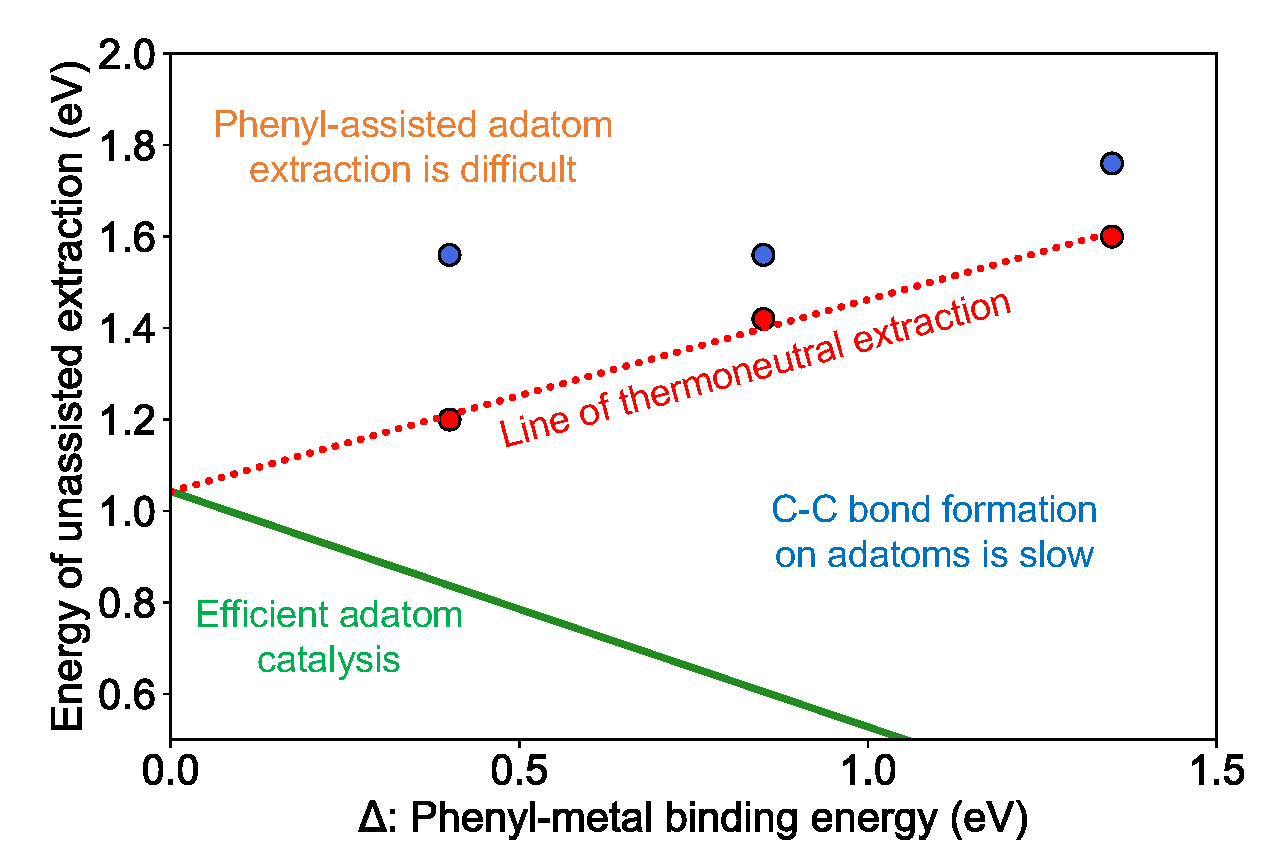
\includegraphics[width=0.48\textwidth]{Fig/conclusion.pdf}
\caption{Conditions for the competitive adatom catalyzed coupling of two phenyl groups. $\Delta$ in the x-axis label refers to the change in the phenyl-metal binding from the ideal suface to adatom. Green lines are lines of constant ratio of the rates of adatom- and surface-catalyzed C--C bond formation (details in \sinfo). The solid green line marks the ratio of 1. %In the right region, adatom catalysis is uncompetitive because adatoms bind phenyl groups too strongly.  In the upper region, adatom catalisys is restricted because the atom extraction is difficult. Remarkably, the DFT determined condition for the thermoneutral assisted adatom extraction -- a prerequisite for competitive adatom catalysis -- is a straight line in this plot.
} 
\label{fig:conclusion}
\end{figure}

\textbf{Implications for adatom catalysis.} 
%
The analysis of the three metals performed in this work raises a tantalizing question whether it is at all possible to find a metal surface capable of catalyzing the Ullmann coupling through an adatom pathway that is faster than the conventional ideal-surface mechanism. 
The preceding discussion of the DFT data reveals that the strengthening of the phenyl-adatom binding relative to the phenyl-surface binding (Fig.~\ref{fig:onlysurface}) is the main parameter that determines the efficiency of both the extraction and adatom-catalyzed C--C bond formation steps (Figure~\ref{fig:onlysurface}b).
The example of Au(111) demonstrates that low strengthening leads to weak extraction assistance, which makes the extraction step uncompetitive. On the other hand, the examples of Ag(111) and Cu(111) show that high strengthening may facilitate the extraction but prohibits the second C--C bond formation step. 

To obviate the dilemma, other parameters of the process must be considered when the surface is chosen or designed. It is reasonable to expect, that the phenyl-assisted extraction can be facilitated without hindering the adatom catalyzed C--C bond formation if metal catalysts with low energy of the unassisted adatom extraction are employed. 
%
Comparing the rates of the biphenyl formation along the adatom and ideal-surface pathways reveals a trend (\sinfo) that allows to estimate that the energy \sout{of the adatom extraction on a clean metal surface} {\zhzh of unassisted adatom extraction on metal surface} cannot exceed \SI{1.0}{\electronvolt} (cf. \SI{1.56}{\electronvolt} for gold) for a competitive adatom-catalyzed coupling of two phenyl groups (Fig.~\ref{fig:conclusion}).
It can be speculated that alloys of copper, silver and gold with different ratio of the components can satisfy this requirement because the lattice incommensurabilities may make atom extraction easier. 

%It is also worth mentioning the analysis presented in Fig.~\ref{fig:conclusion} can greatly reduce the number of DFT calculations necessary to predict co
%Knowing this upper bound can greatly facilitate computational screening of metals for the efficient trap-free adatom catalysis since the only DFT calculations needed are those for clean metal surfaces. The screening accuracy can be further improved if the horizontal position on the figure is also available from additional DFT calculations for a candidate metal. For example, inert metals like gold cannot have more than \SI{0.84}{\electronvolt} energy of the unassisted adatom extraction whereas for metals like silver this limit is even more restrictive \SI{0.60}{\electronvolt}. 

The data presented in this work suggests that, for many other C--C bond forming reactions on metal surfaces, plots similar to Fig.~\ref{fig:conclusion} can have much wider areas of competitive adatom catalysis and that constructing such plots can facilitate investigation of catalytic mechanisms. 

%\section*{Conclusions}

To conclude, the role of adatoms in the coupling of iodo-, bromo- and chlorobenzene on the Cu(111), Ag(111) and Au(111) surfaces was investigated using DFT modeling. For all three metals, it was found that the energy of the phenyl-assisted adatom creation is significantly lower than the energy of the clean-surface unassisted adatom creation. In the most dramatic example of Cu(111), the two energies are \SI{0.16}{\electronvolt} and \SI{1.76}{\electronvolt}, respectively. In the case of the phenyl-assisted metal atom extraction, the energy cost of breaking metal-metal bonds is almost completely offset by the increased binding of the phenyl groups to the extracted metal atom. This effect is also responsible for the low phenyl-assisted extraction barriers computed for all three metals (\SI{0.71}{\electronvolt} Cu, \SI{0.43}{\electronvolt} Ag, \SI{0.36}{\electronvolt} Au). 

Quantifying the strengthening of phenyl-adatom bonds for all three metals revealed its strong correlation with the increased activation barrier of the C--C bond formation on adatoms. In the case of Cu(111) and Ag(111), the adatom-catalyzed C--C bond formation barriers are found to be extremely high (\SI{1.78}{\electronvolt} Cu, \SI{1.52}{\electronvolt} Ag) rendering this adatom-based catalytic mechanism impossible despite the ease of the phenyl-assisted adatom extraction. 
%These high barriers also mean that phenyl-bonded adatoms form only fleetingly on Cu(111) and Ag(111) before recombining with their vacancies and undergoing the regular ideal-surface C--C coupling. This competition between adatom and ideal-surface pathways makes adatom-containing organometallic bridges unlikely to be observed by STM or AFM. 
In stark contrast to Cu and Ag, the C--C bond formation barrier on Au adatoms is only \SI{0.20}{\electronvolt}. Nevertheless, the adatom catalysis on Au is still slower than the ideal-surface catalysis because it is the extraction step that hinders it in this case.

DFT is used to predict the behavior of not only the phenyl-extracted adatoms but also the adatoms that already exist on metal surfaces, for example, around steps and kinks. On Cu(111) and Ag(111), pre-existing adatoms bind phenyl groups so strongly that they are unable to catalyze the subsequent C--C bond formation. Without the possibility to recombine with a vacancy these organometallic adatom states form low-energy traps. In contrast, pre-existing Au adatoms are not expected to form such traps as they catalyze the C--C bond formation almost as efficiently as ideal-surface atoms. This implies that the Ullmann polymerization on Au(111) can produce fewer defects in surface-assembled nanostructures than the same process on Ag(111) and Cu(111)~\cite{ullmann_65}.

This work have important implications. The systematic comparison of the reaction energetics on ideal surfaces and adatoms allows to make rational predictions about the influence of other defects, such as terrace edges and kinks, on the Ullmann coupling reactions, facilitating investigation of their mechanisms.
Fundamental analysis of the systematic DFT data can also advance design of effective adatom catalysts for a variety of on-surface reactions. As demonstrated in this work, one strategy to design adatom catalyzed reactions is to focus on metals with low adatom-vacancy formation energies while a complementary strategy would be to find reactants that bind to adatoms and surface atoms equally strongly. 

\ifdefined\ACSNANO

\section*{Computational Methods}

The (111) metal surfaces were modeled with slabs containing 192 metal atoms arranged in four 8 $\times$ 6 atomic layers. \SI{10}{\angstrom} of vacuum was added in the direction normal to the surface to ensure weak interaction between periodic images of the slab. The size of the slabs in the lateral directions was $20.55 \times 13.35$~\si{\angstrom} for Cu, $22.84 \times 14.82$~\si{\angstrom} for Ag, and $22.47 \times 14.60$~\si{\angstrom} for Au. It is assumed that the presence of the vacancy does not affect the state energetics drastically and, therefore, the vacancy-containing models are used to model pre-existing adatoms. 

DFT calculations were performed using Vienna \emph{ab initio} simulation package (VASP)~\cite{ullmann_131, ullmann_132, ullmann_133, ullmann_134}. The dispersion-corrected~\cite{ullmann_136, ullmann_137} Perdew-Burke-Ernzerhof (PBE) generalized gradient approximation~\cite{ullmann_139} was used as the exchange-correlation functional. 
Spin-polarized electronic states were modeled using a plane wave basis set with the energy cut-off set at \SI{800}{\electronvolt}.
The projector augmented wave formalism was used to describe interactions of atomic cores with valence electrons. The integration over the Brillouin zone was performed using the $3\times 3 \times1$ Monkhorst-Pack $k$-point mesh. 

Atomic positions were optimized until the maximum force on atoms decreased below \SI{0.02}{\electronvolt\per\angstrom}. 
Transition state structures were located using the climbing-image nudged elastic band (NEB) with the VTST code~\cite{ullmann_59}. 
In NEB calculations, an improved initial guess~\cite{ullmann_60, ullmann_99} for the minimum energy path was used and the positions of atoms were relaxed until the maximum force dropped below \SI{0.1}{\electronvolt\per\angstrom}.

%{\comm RZK0804: Energy vs enthalpy.}


\fi

\section*{Acknowledgement}

The research was funded by the Natural Sciences and Engineering Research Council of Canada (NSERC) through Discovery Grant (RGPIN-2016-0505) and by Tri-agency Institutional Programs Secretariat through New Frontiers in Research Fund (NFRFE-2018-00852). The authors are grateful for computer resources allocated under the CFI John R. Evans Leaders Fund program.

\section*{\sinfo}

%The Supporting Information is available free of charge at (website)
Formation of organometallic intermediates on Cu(111); characterization of the intermediates in the dehalogenation step on Cu(111); minimum experimentally measured temperatures necessary for the completion of the Ullmann coupling steps; characterization of the intermediates in the C--C bond formation step along the ideal-surface and two adatoms pathways; conditions for competitive adatom catalysis.

%%%%%%%%%%%%%%%%%%%%%%%%%%%%%%%%%%%%%%%%%%%%%%%%%%%%%%%%%%%%%%%%%%%%%
%%A listing of the contents of each file supplied as Supporting Information
%%should be included. For instructions on what should be included in the
%%Supporting Information as well as how to prepare this material for
%%publications, refer to the journal's Instructions for Authors.

%%The following files are available free of charge.
%%\begin{itemize}
%%  \item Filename: brief description
%%  \item Filename: brief description
%%\end{itemize}
%%%%%%%%%%%%%%%%%%%%%%%%%%%%%%%%%%%%%%%%%%%%%%%%%%%%%%%%%%%%%%%%%%%%%
%\end{suppinfo}

%\begin{tocentry}
%
%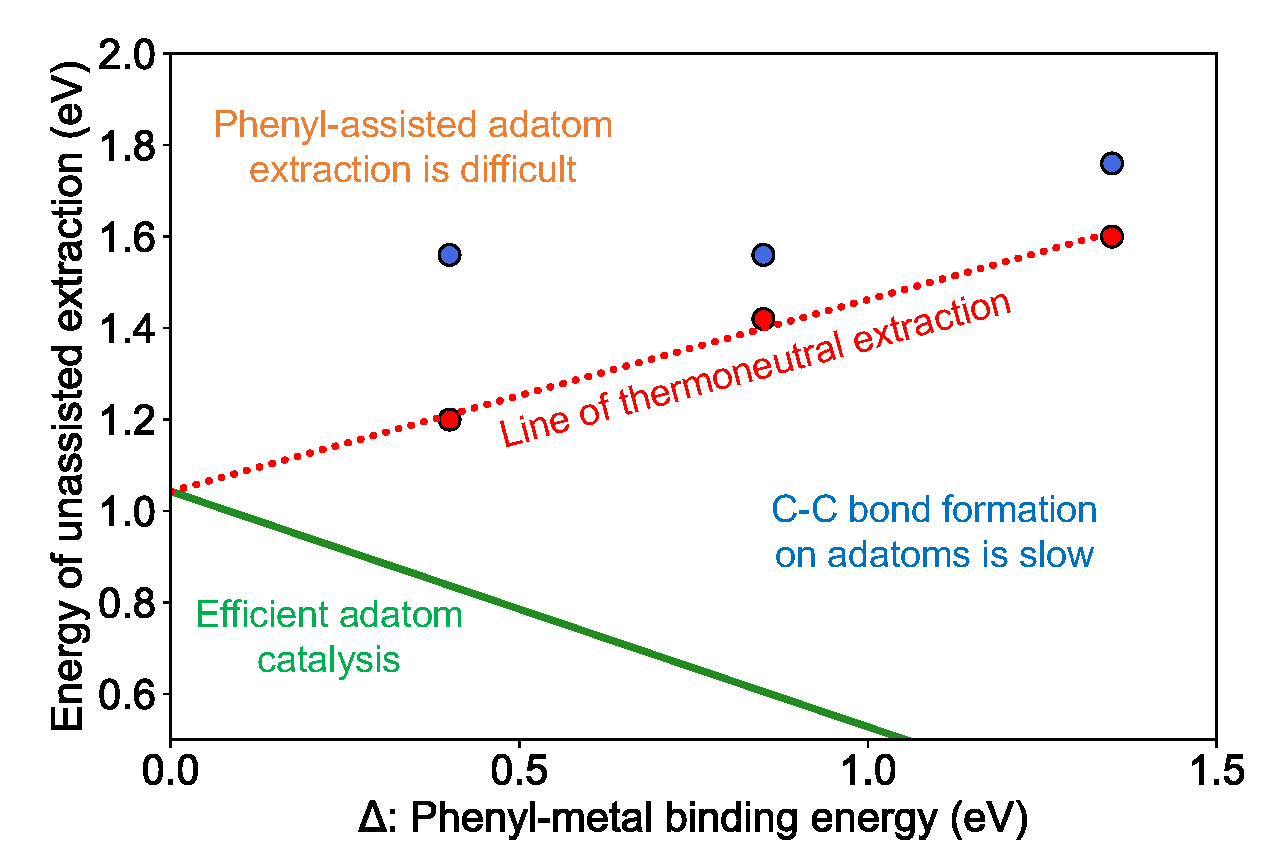
\includegraphics[width=0.62\textwidth]{Fig/conclusion.pdf}\newline
%This TOG is temporary.
%
%\end{tocentry}

%\nocite{*}

%%%%%%%%%%%%%%%%%%%%%%%%%%%%%%%%%%%%%%%%%%%%%%%%%%%%%%%%%%%%%%%%%%%%%
%% The appropriate \bibliography command should be placed here.
%% Notice that the class file automatically sets \bibliographystyle
%% and also names the section correctly.
%%%%%%%%%%%%%%%%%%%%%%%%%%%%%%%%%%%%%%%%%%%%%%%%%%%%%%%%%%%%%%%%%%%%%

%\pagebreak

\bibliographystyle{achemso}
\bibliography{references}

\pagebreak

\end{document}








